% KAFCA documentation for the Kassiopeia Guide
% B.Leiber email: benjamin.leiber@kit.edu
\section{Ferenc's Field Simulation: KAFCA}\label{sec:KAFCA}
\subsection{Magnetic field calculation with the Legendre polynomial expansion}
%% =============================
	\subsubsection{Elliptic Integrals}
	  The main components generating magnetic fields in the KATRIN experiment are circular coils and superconducting solenoids. These are simple circular current loops, that have a rotational symmetry axis (compare fig. \ref{fig:current loop}). 
	  \begin{figure}[h]
		\centering 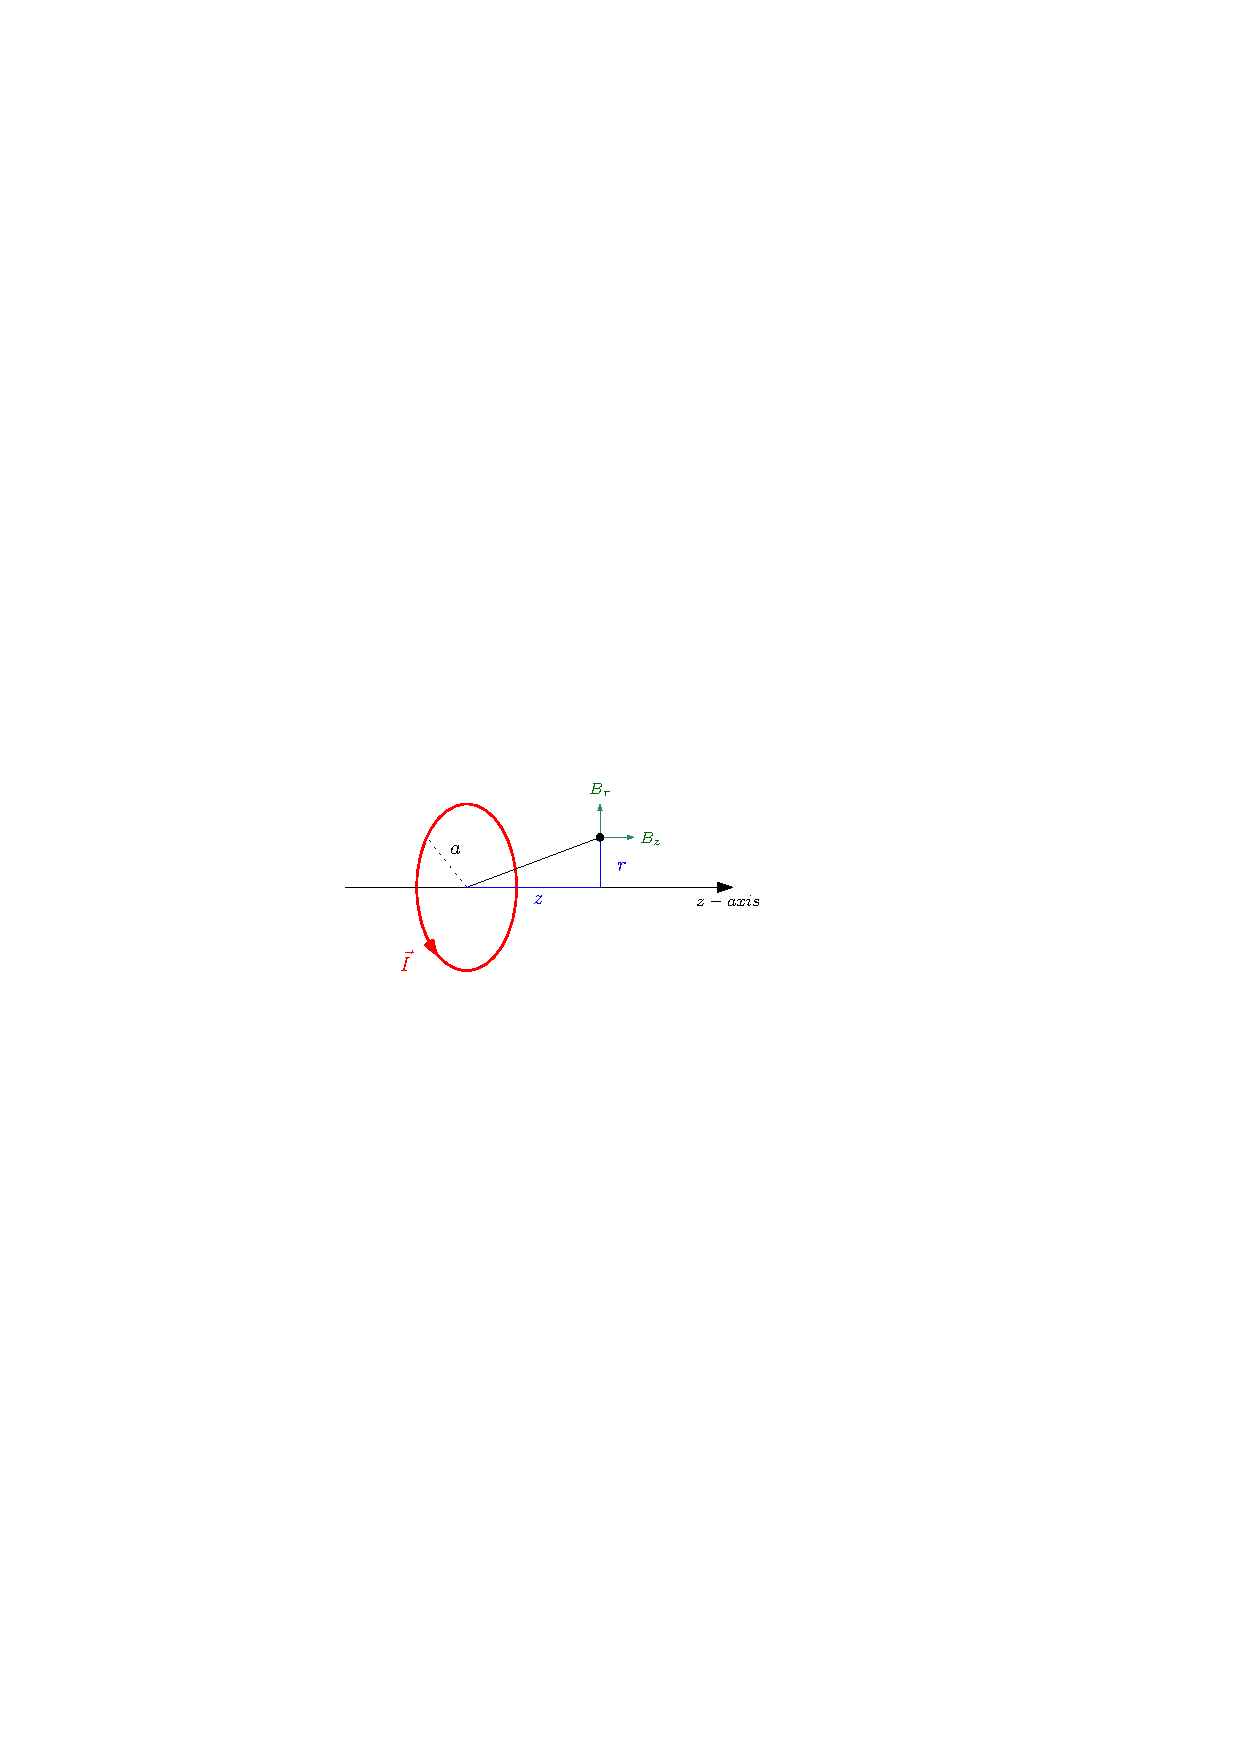
\includegraphics[width=0.7\textwidth]{images/KAFCAFigures/current_loop.pdf}
		\caption{A loop with the radius $a$ and the current $\vec{I}$ running through it, induces a magnetic field $\vec{B}$}
		\label{fig:current loop}
	  \end{figure}\\
	  The Biot-Savart law \eqref{eq:biot savart} for a thin coil can be expressed in terms of the complete elliptic integrals:
%====================	
	%elliptic Integrals
	\begin{equation}
		\begin{aligned}
			K(k) &= \int\limits_{0}^{\frac{\pi}{2}} \frac{\mathrm d\varphi}{\sqrt{1-k^{2}\sin^{2}\varphi}} & \text{(I)}\\
			E(k) &= \int\limits_{0}^{\frac{\pi}{2}} \mathrm{d}\varphi\sqrt{1-k^{2}\sin^{2}\varphi} & \text{(II)} \\
			\Pi(c,k) &= \int\limits_{0}^{\frac{\pi}{2}} \frac{\mathrm d\varphi}{(1-c^{2}\sin^{2}\varphi)\sqrt{1-k^{2}\sin^{2}\varphi}}  & \text{(III)}
		\end{aligned}
		\label{eq:complete elliptic integrals}
	\end{equation}
	They can be used for an analytical computation of the magnetic field \cite{jackson}:
	\begin{equation}
		\begin{aligned}
			B_{r} &= \frac{I}{c} \frac{2z}{r\sqrt{(a+r)^{2}+z^{2}}} \left[ -K(k) + \frac{a^{2}+r^{2}+z^{2}}{(a+r)^{2}+z^{2}}E(k)\right] \\
			B_{\varphi} &= 0 \\
			B_{z} &= \frac{I}{c} \frac{2}{r\sqrt{(a+r)^{2}+z^{2}}} \left[ K(k) + \frac{a^{2}-r^{2}-z^{2}}{(a+r)^{2}+z^{2}}E(k)\right]
		\end{aligned}
		\label{eq:magnetic field elliptic integrals}
	\end{equation}
	where $k^2 = \frac{4ar}{z^2 + \left(a+r\right)^2}$. For real coils, with a finite length, the third integral is also needed for a description of the magnetic field. Usually, $K(k)$, $E(k)$ and $\Pi(c,k)$ are expressed via Carlson's elliptic integrals $R_F$, $R_J$, $R_D$ \cite{numericalrecipes}: 
	\begin{equation}
		\begin{aligned}
			K(k) &= (R_{F},0, 1-k^{2},1)\\
			E(k) &= (R_{F},0, 1-k^{2},1) - k^{2}\frac{1}{3}(R_{D},0, 1-k^{2},1) \\
			\Pi(c,k) &= (R_{F},0, 1-k^{2},1) - c^{2}\frac{1}{3}(R_{J},0, 1-k^{2},1,1-c^{2})
		\end{aligned}
		\label{eq:complete elliptic integrals through carlson}
	\end{equation}
	These solutions are valid everywhere and hence, the magnetic field can even be calculated inside the coils. In addition, Carlson's elliptic integrals offer a relatively fast numerical computation method. But still a numerical integration is necessary, which usually means summing over many numbers. To speed things up, a solution has to be found that is fast to compute: the zonal-harmonics are appropriate solutions for axisymmetric coils. They can be computed fast and offer a variable precision, depending on the number of expansion orders that are considered.
      \subsubsection{Zonal Harmonic Expansion}
	The magnetic field at a point $\vec{p}(r,z)$ close to the symmetry axis, can be expressed in terms of the Legendre polynomial expansion and its derivatives at the point $z_0$ that lies on the symmetry axis, a so called sourcepoint. In case the distance of the field-point to the sourcepoint is smaller than the minimal distance of the sourcepoint to the coil body ($\rho < \rho_{cen}$, see fig. \ref{fig:central convergence radius}), the magnetic field is given by the so called central expansion:
	\begin{equation}
		\begin{aligned}
			B_r &= -s\sum_{n=1}^{\infty} \frac{B_{n}^{cen}}{n+1} \left(\frac{\rho}{\rho_{cen}}\right)^{n}P'_n(u) \\
			B_{\varphi} &= 0 \\
			B_z &= \sum_{n=0}^{\infty} B_{n}^{cen}\left(\frac{\rho}{\rho_{cen}}\right)^{n}P_n(u) \\
			&\text{with} \quad u = \cos\theta \quad \text{and} \quad s = \sin\theta
		\end{aligned}
		\label{eq:central polynomial expansion}
	\end{equation}
	with $B_{n}^{cen}$ being the central source coefficients and $P_{n}$ the Legendre polynomials. The minimal distance between the sourcepoint and the coil $\rho_{cen}$ is usually called central convergence radius and equation \eqref{eq:central polynomial expansion} is only valid within.
	  \begin{figure}[h]
		\centering 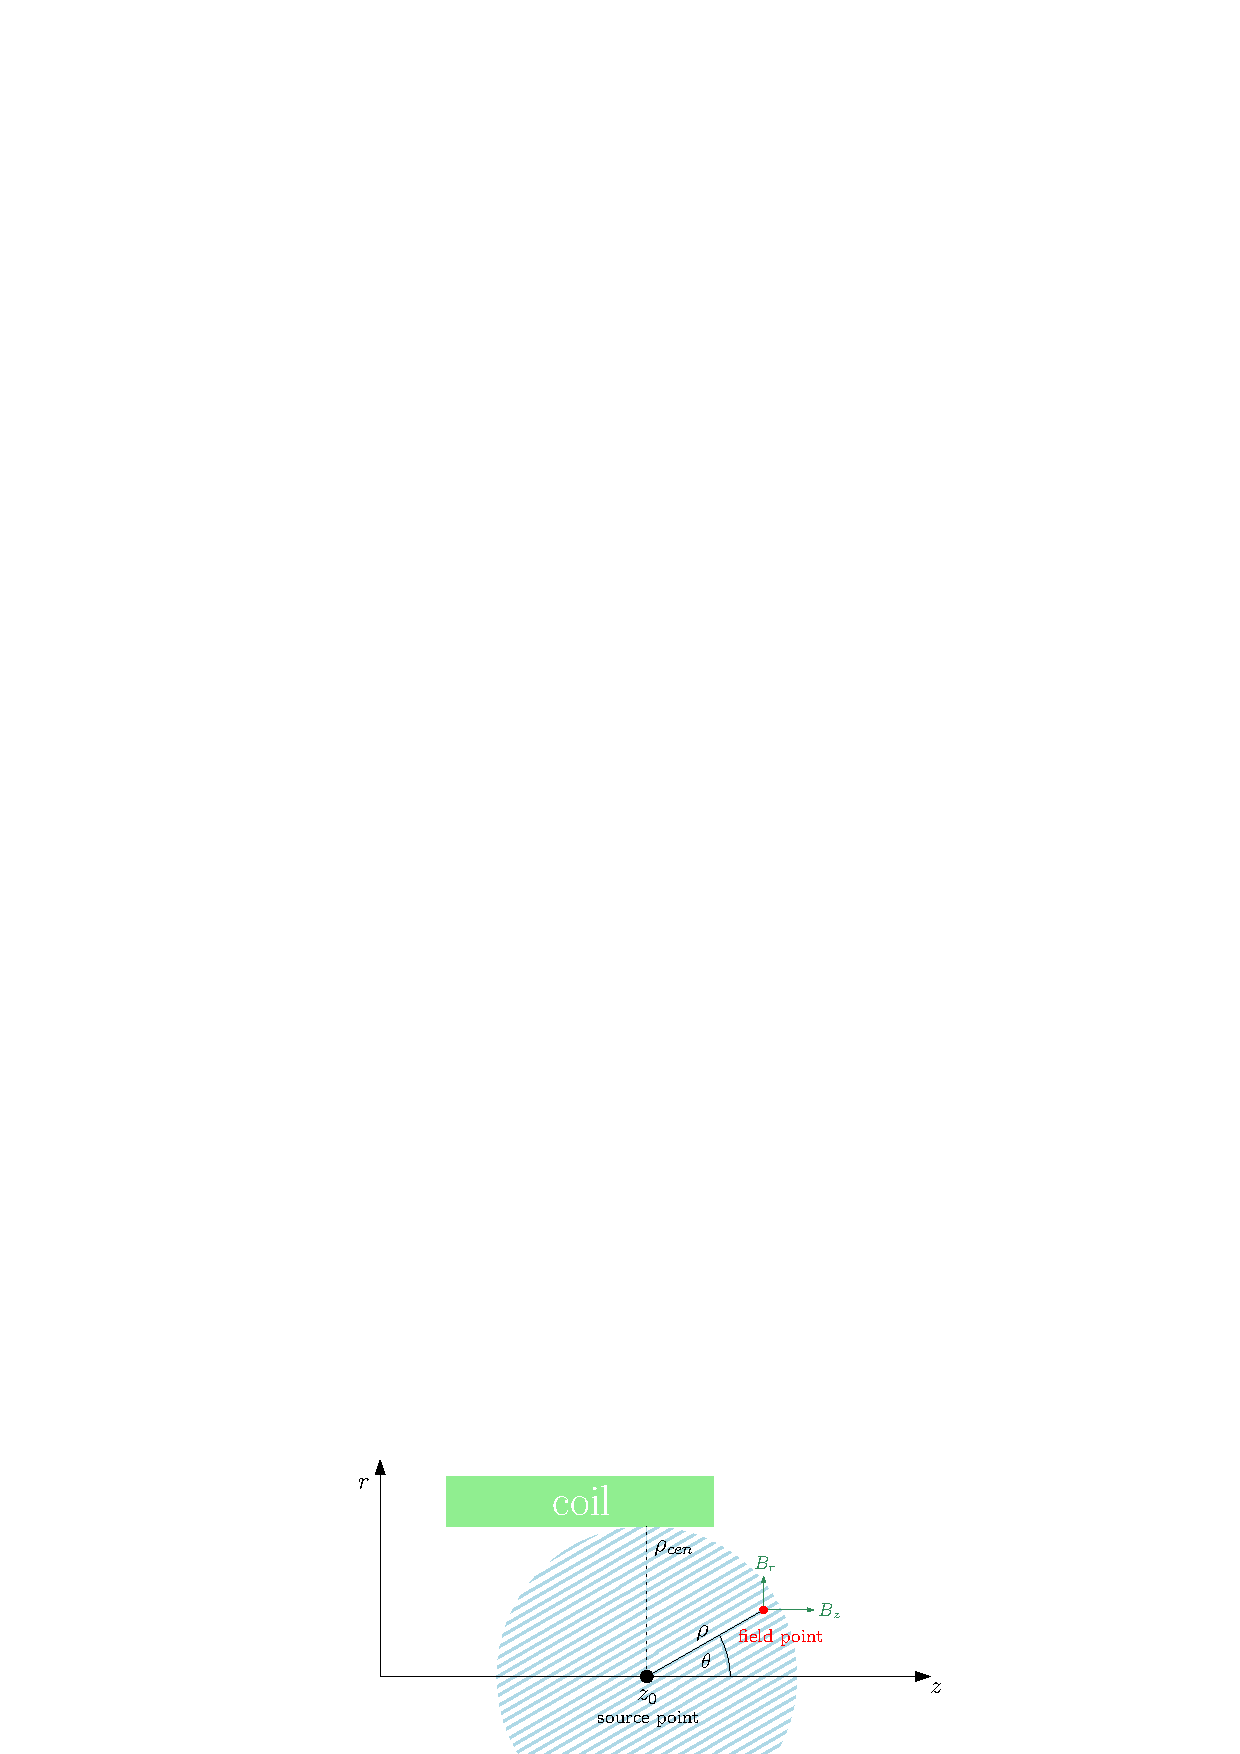
\includegraphics[width=0.7\textwidth]{images/KAFCAFigures/legendre_central.pdf}
		\caption{Convergence radius of the central expansion.}
		\label{fig:central convergence radius}
	  \end{figure}
	  \\
	As we want to know the magnetic field outside of the convergence radius too, a second polynomial expansion has to be introduced. This remote expansion is only valid for distances to the sourcepoint greater than the remote convergence radius $\rho_{rem}$, which is the maximal distance of the sourcepoint to the coil ($\rho > \rho_{rem}$, see fig. \ref{fig:remote convergence radius}). The magnetic field is then defined by the remote expansion:
	\begin{equation}
		\begin{aligned}
			B_r &= s\sum_{n=2}^{\infty} \frac{B_{n}^{rem}}{n} \left(\frac{\rho_{rem}}{\rho}\right)^{n+1}P'_n(u) \\
			B_{\varphi} &= 0 \\
			B_z &= \sum_{n=2}^{\infty} B_{n}^{rem}\left(\frac{\rho_{rem}}{\rho}\right)^{n+1}P_n(u) %\\
			%&\text{with} \quad u = \cos\theta \quad \text{and} \quad s = \sin\theta
		\end{aligned}
		\label{eq:remote polynomial expansion}
	\end{equation}
	with $B_{n}^{rem}$ being the remote source coefficients.
	\begin{figure}[h]
		\centering 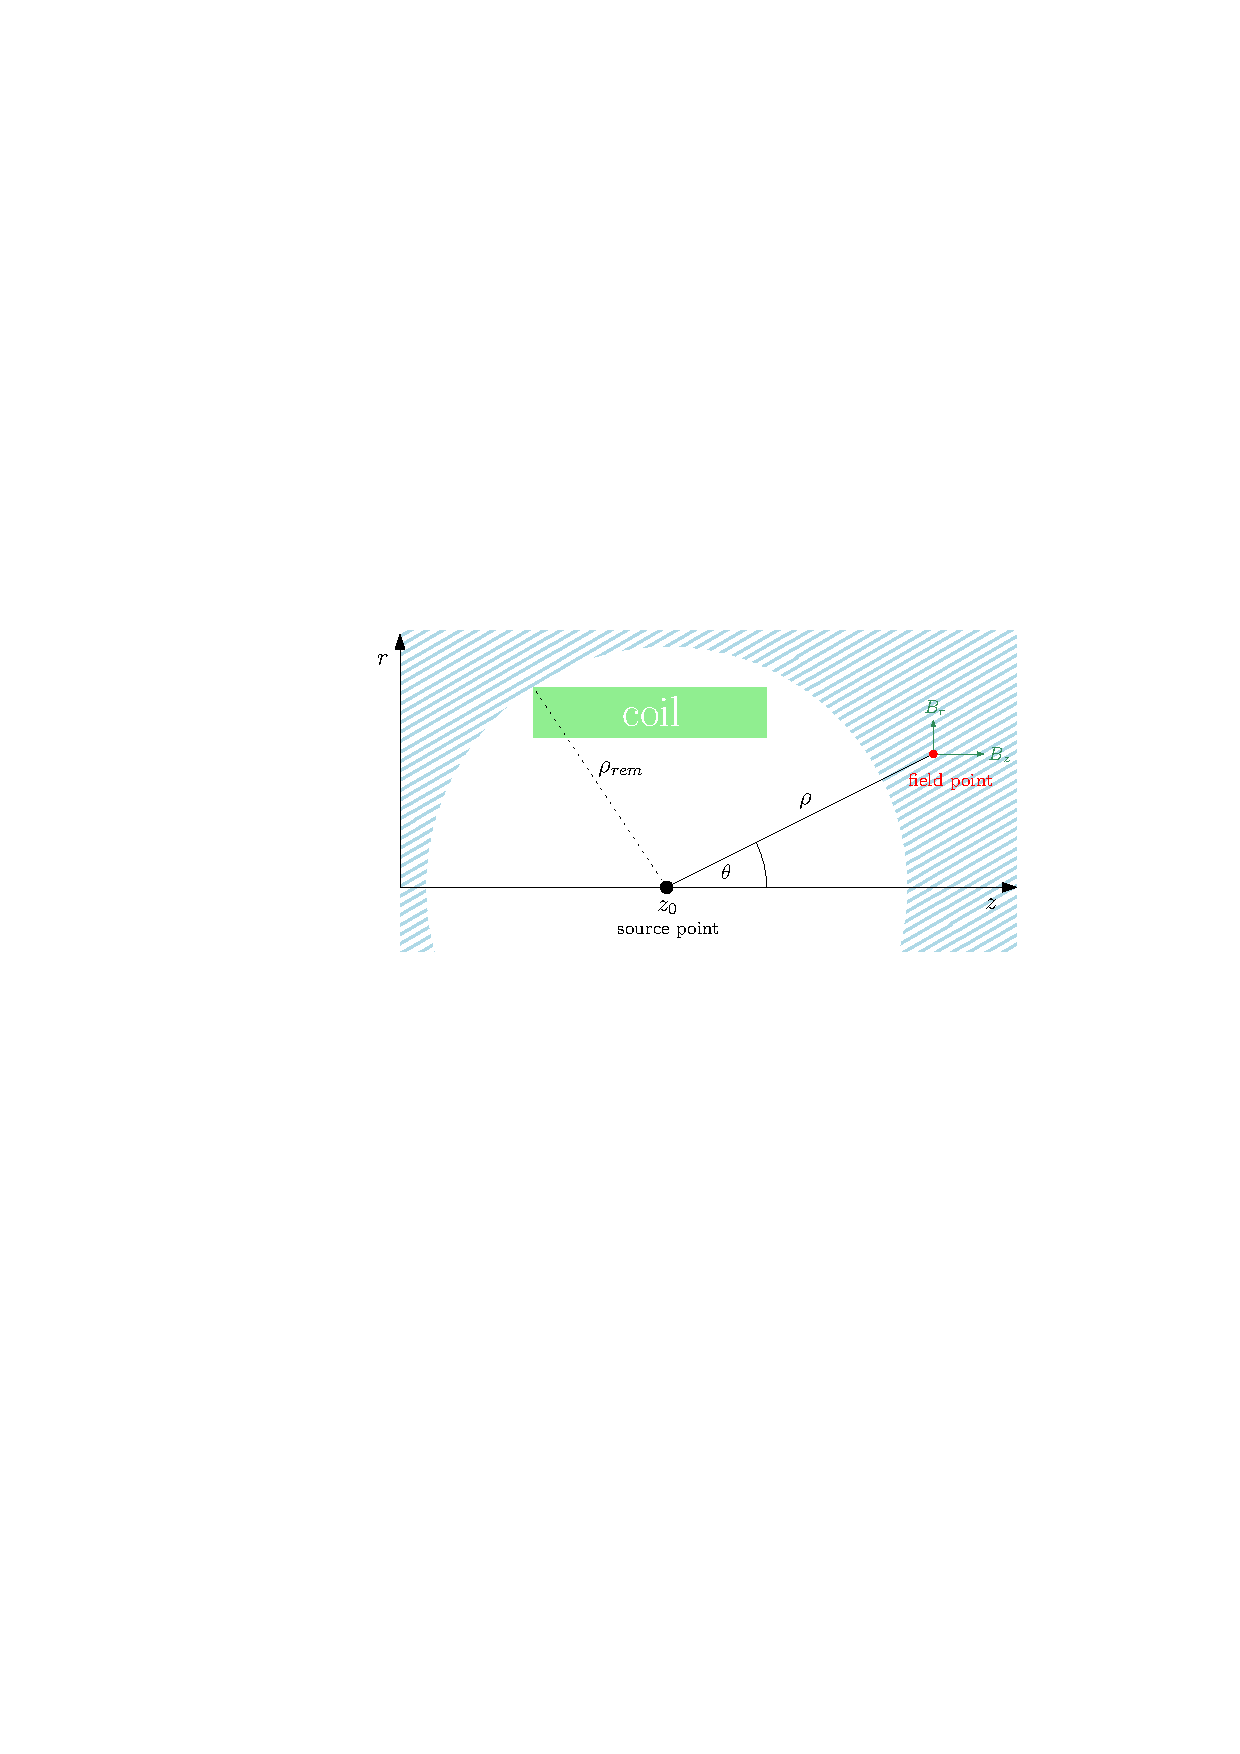
\includegraphics[width=0.7\textwidth]{images/KAFCAFigures/legendre_remote.pdf}
		\caption{Convergence radius of the remote expansion.}
	  \label{fig:remote convergence radius}
	\end{figure}
	\\
	These expansions now allow a very fast field-computation nearly everywhere in the system. They are not valid close to and inside the coils, so elliptic integrals have to be used here.
      %\subsubsection{Implementation}
      \subsubsection{Application}
	For the description of a system of multiple coils, the convergence radii are determined by the closest, respectively the most remote coil (see fig. \ref{fig:two coils one sourcepoint}).
	\begin{figure}[htbp]
	      \centering
	      %\begin{minipage}{0.7\textwidth}
	      \begin{minipage}{0.49\textwidth}
		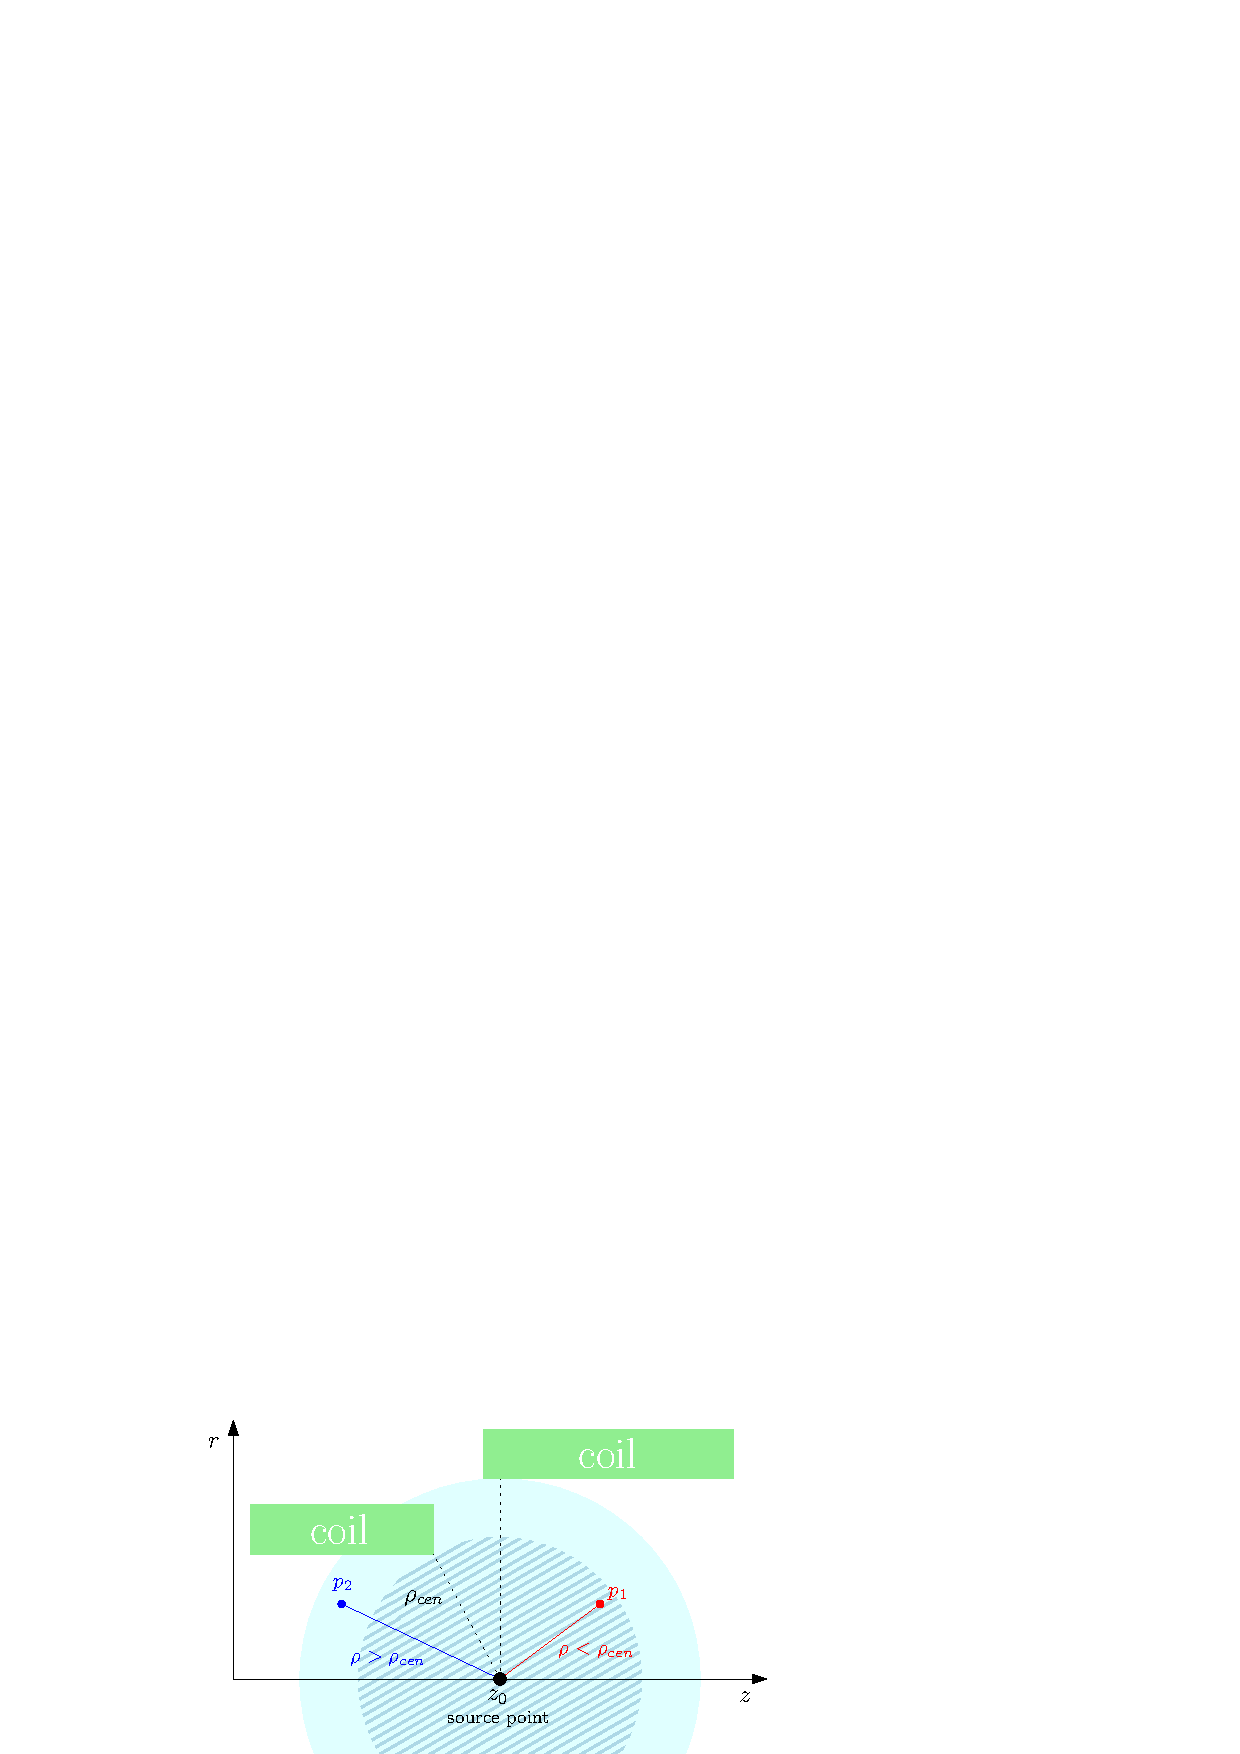
\includegraphics[width=0.95\textwidth]{images/KAFCAFigures/two_coils_central.pdf}
	      \end{minipage}
	      %\\
	      %\begin{minipage}{0.85\textwidth}
	      \begin{minipage}{0.49\textwidth}
		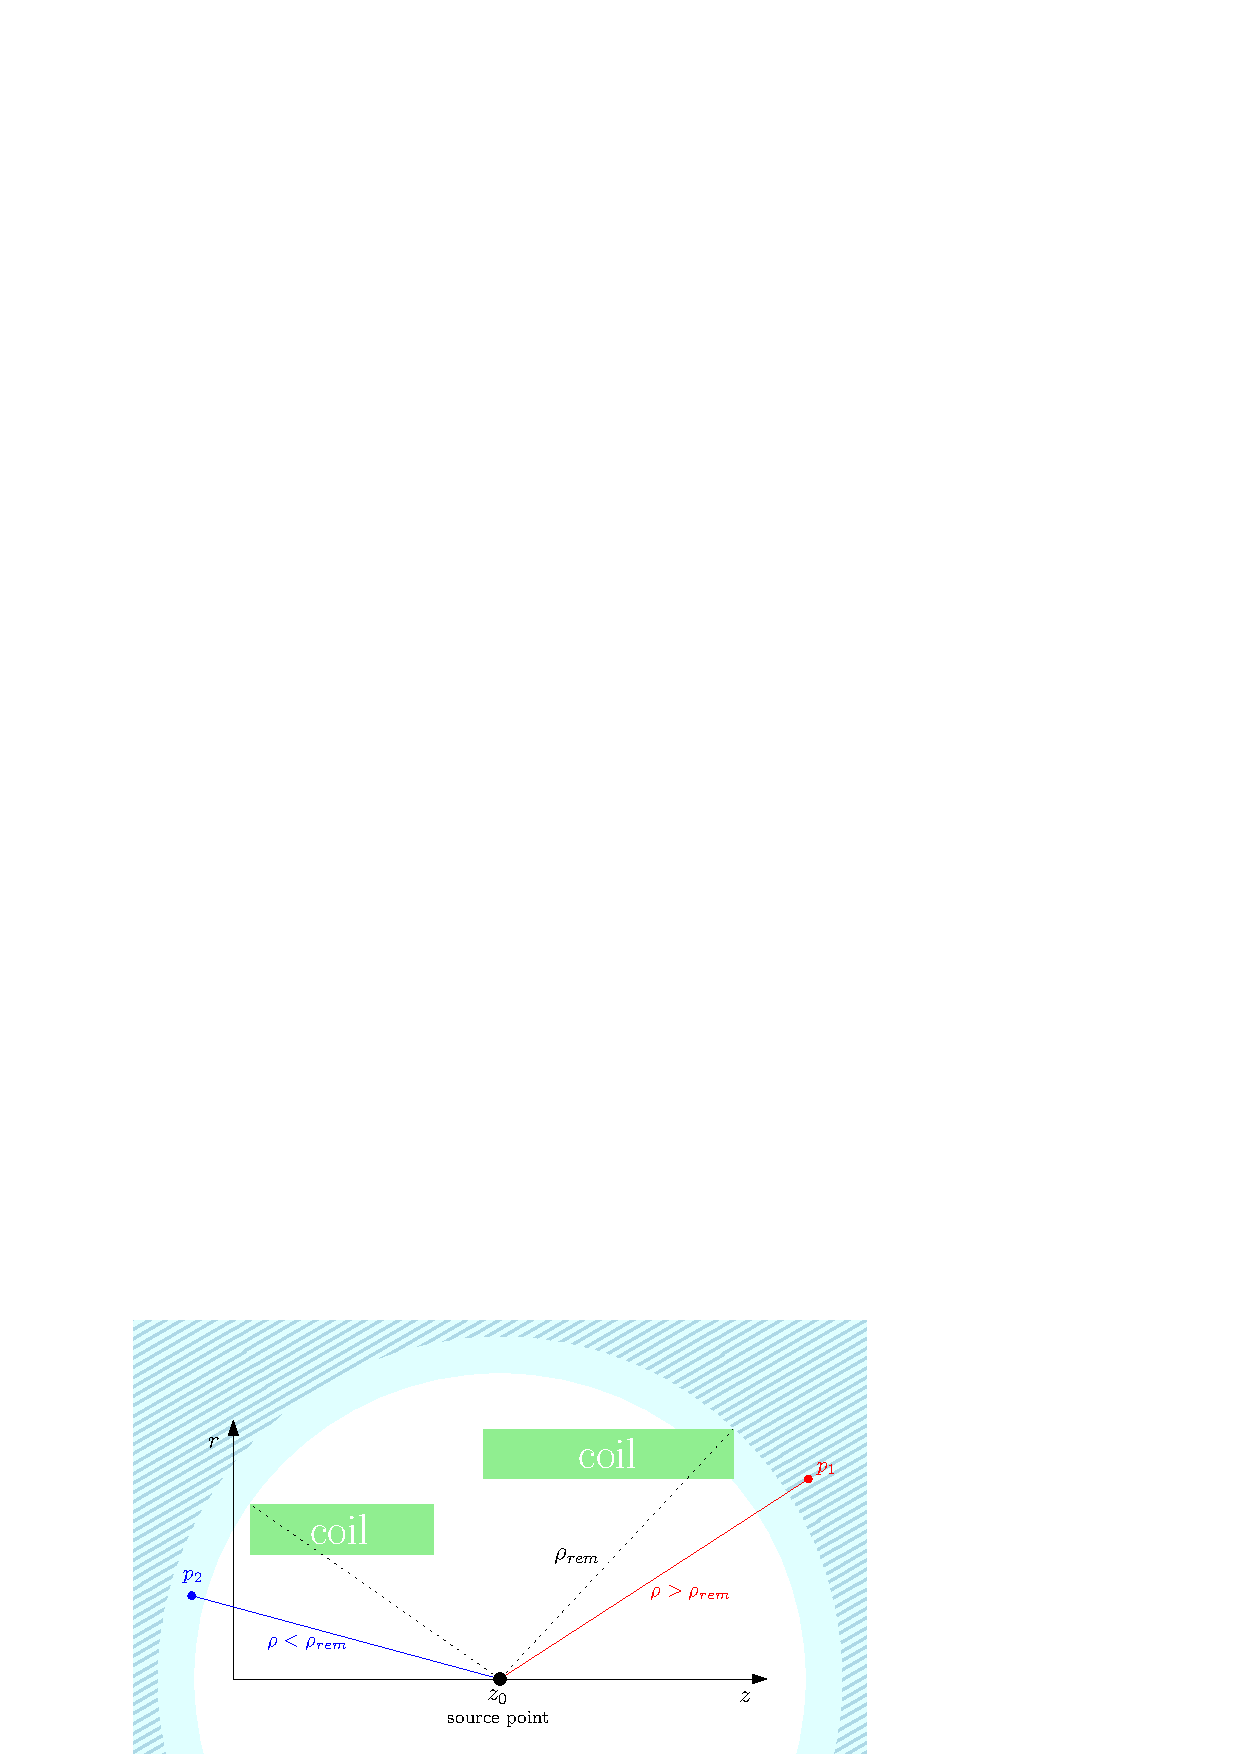
\includegraphics[width=0.95\textwidth]{images/KAFCAFigures/two_coils_remote.pdf}
	      \end{minipage}
	      \caption{Central convergence radius (top) and remote convergence radius (below), with two coils using only one sourcepoint. The expansions converge in $p_1$ but not in $p_2$.}
	      \label{fig:two coils one sourcepoint}
	\end{figure}
	To cover a larger area the amount of sourcepoints can simply be increased as shown in figure\ref{fig:two coils two sourcepoints}.
	\begin{figure}[htbp]
	      \centering
	      %\begin{minipage}{0.7\textwidth}
	      \begin{minipage}{0.49\textwidth}
		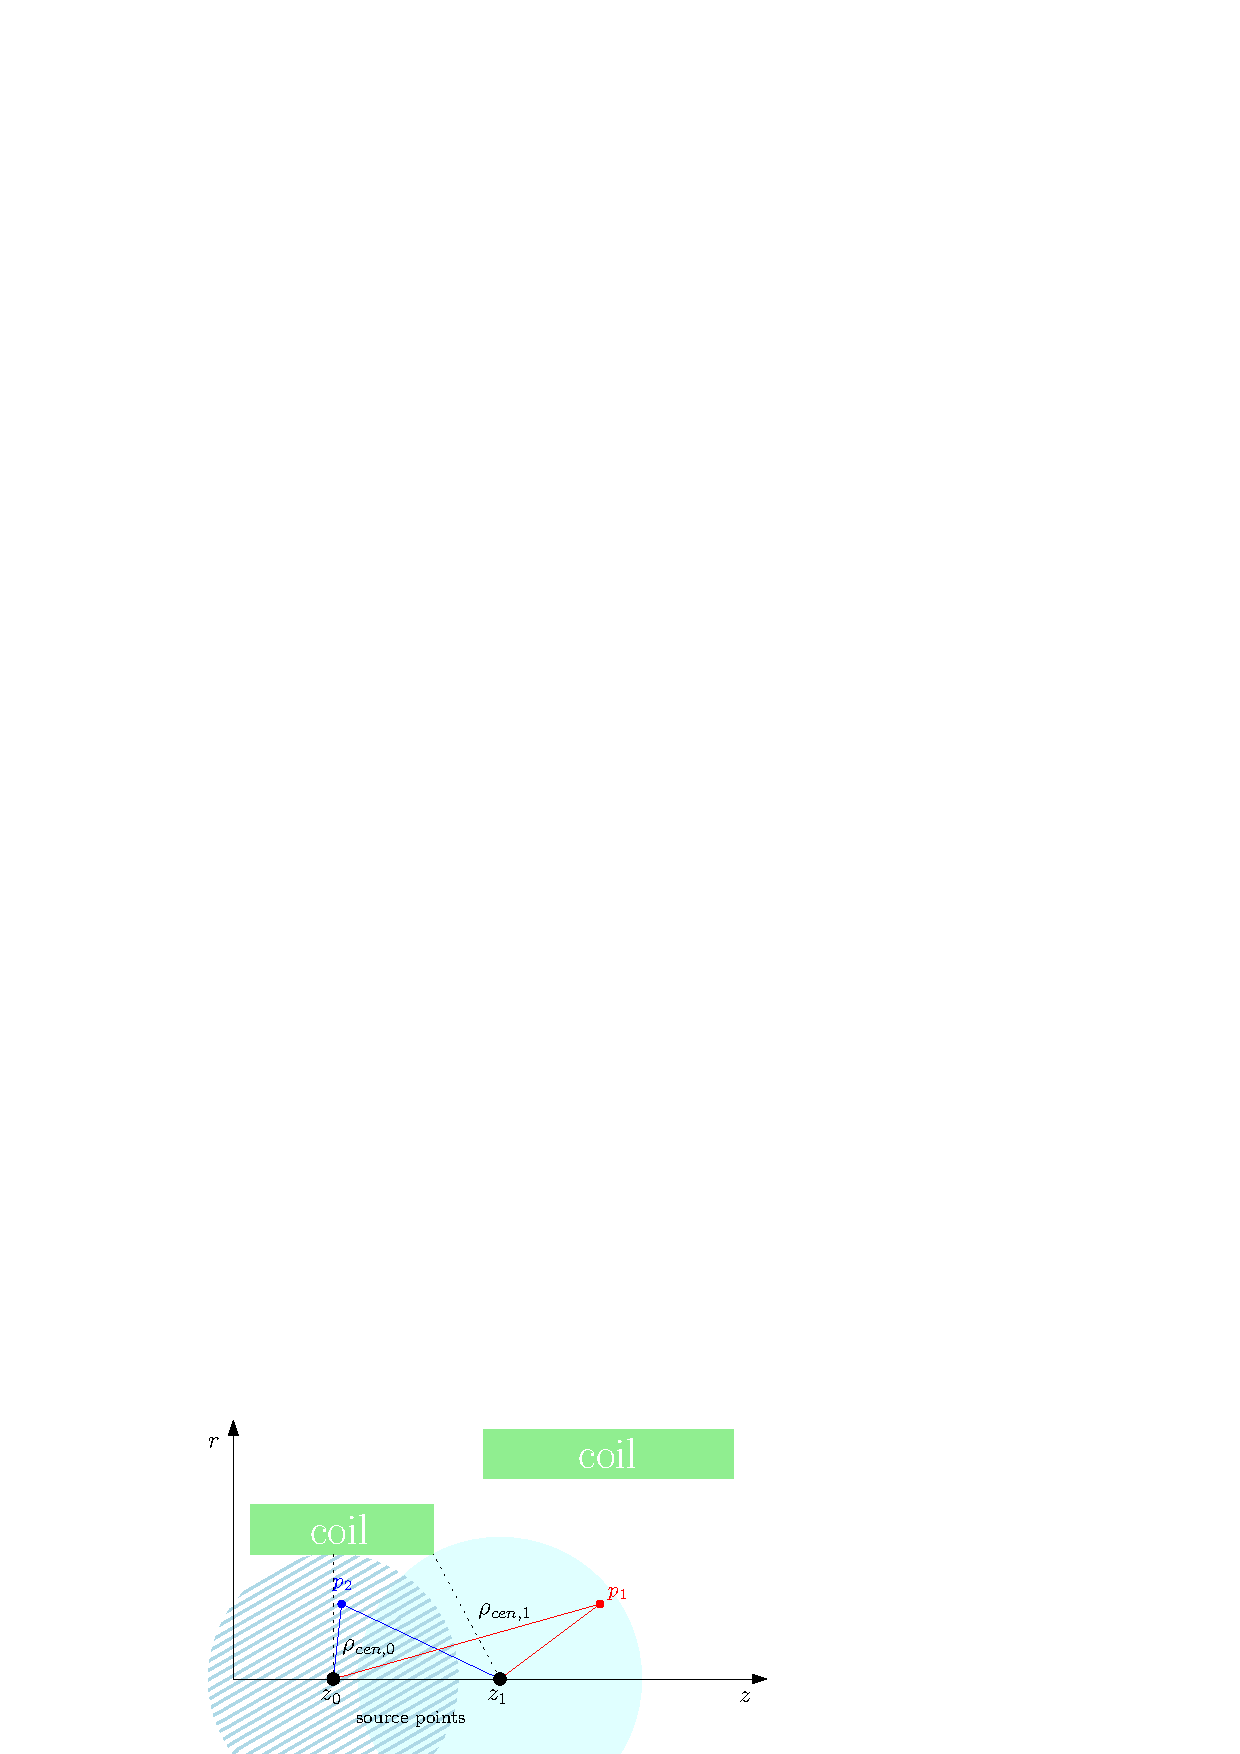
\includegraphics[width=0.95\textwidth]{images/KAFCAFigures/two_coils_central_two_sp.pdf}
	      \end{minipage}
	      %\\
	      %\begin{minipage}{0.85\textwidth}
	      \begin{minipage}{0.49\textwidth}
		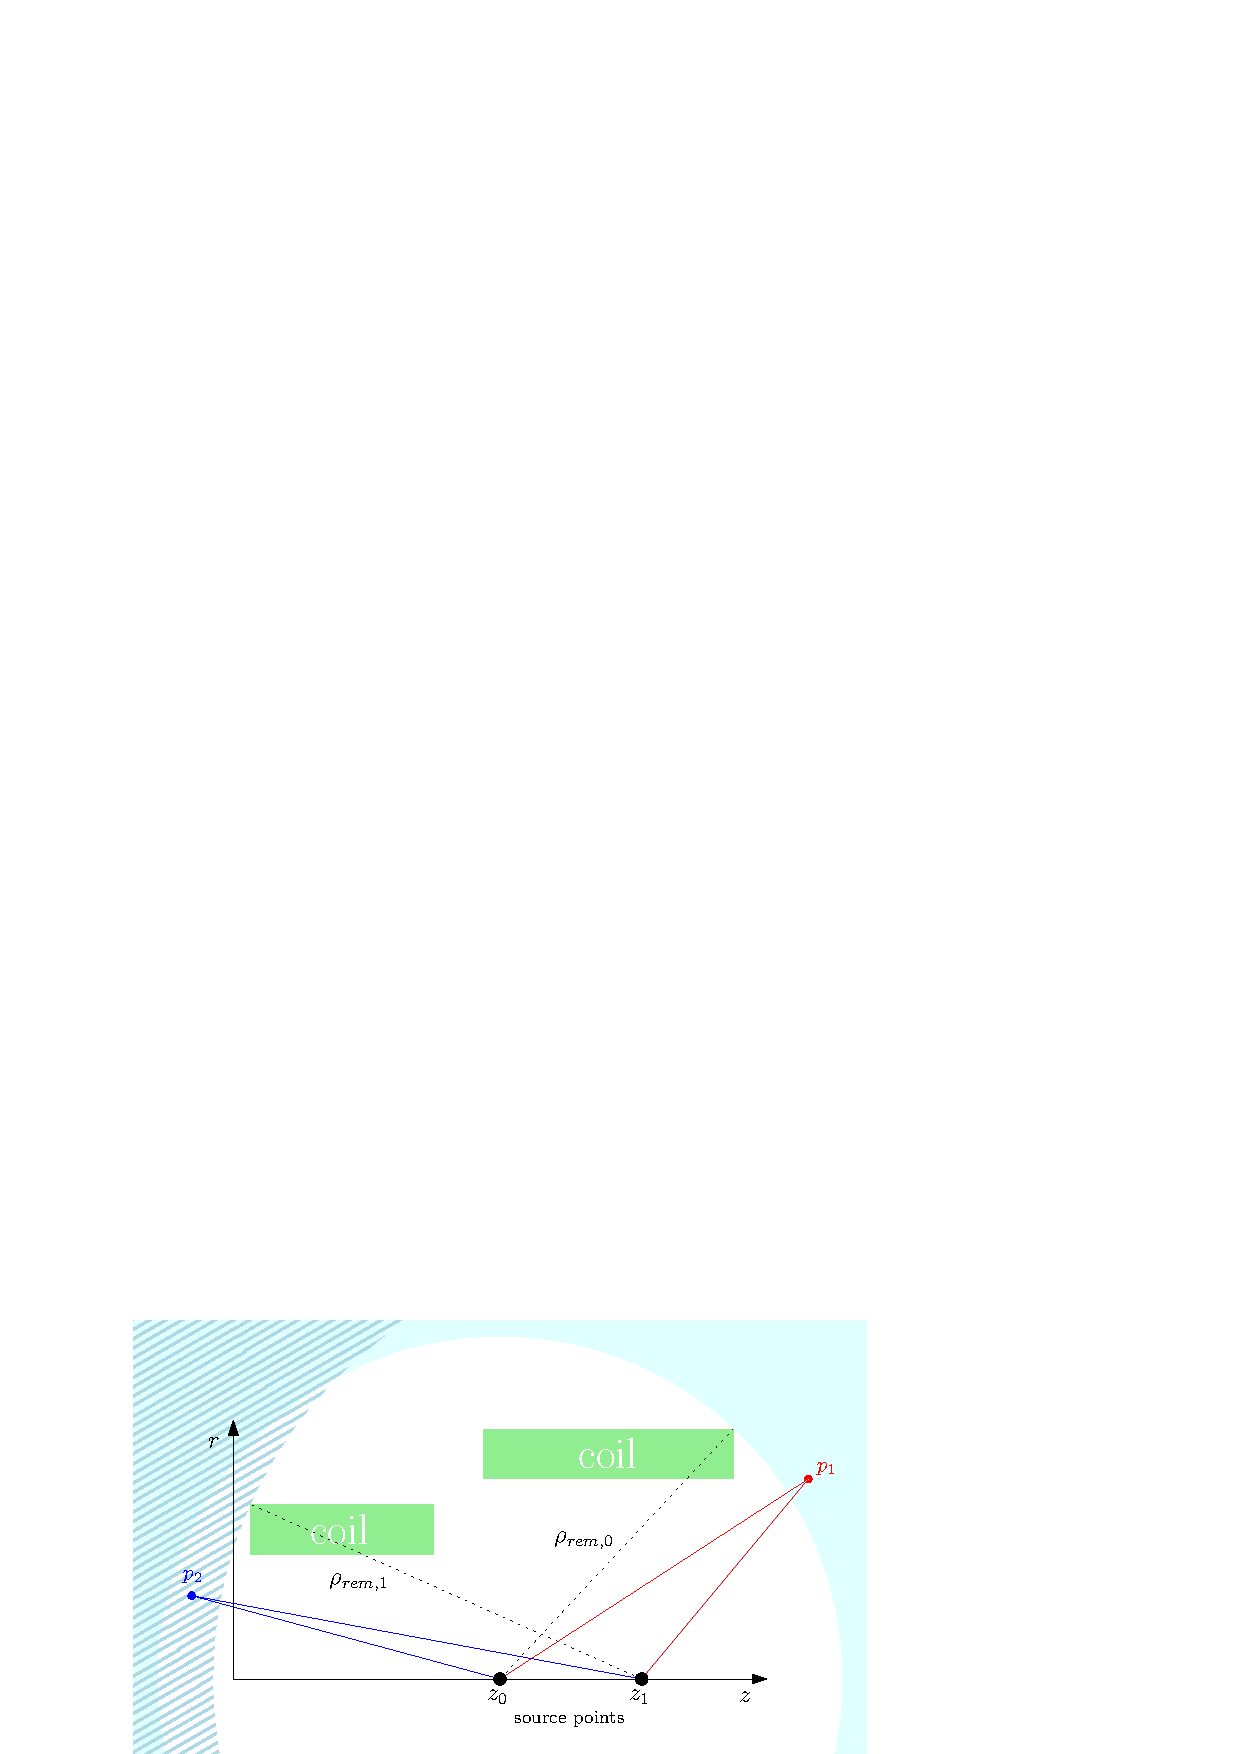
\includegraphics[width=0.95\textwidth]{images/KAFCAFigures/two_coils_remote_two_sp.pdf}
	      \end{minipage}
	      \caption{With the additional sourcepoints, it is now possible to compute the magnetic field in both $p_1$ and $p_2$ with the polynomial expansion.}
	      \label{fig:two coils two sourcepoints}
	\end{figure}
	Another benefit of having several sourcepoints is a faster computation, as the polynomial expansion converges faster if the fractions $\frac{\rho}{\rho_{cen}}$ and $\frac{\rho_{rem}}{\rho}$ are smaller. By choosing the sourcepoint with the smallest fraction for the field point to be calculated, a lot of computation time can be saved.
	\\
	In preparation for the polynomial expansion, the source coefficients $B_{n}^{cen}$ and $B_{n}^{rem}$ need to be computed at every sourcepoint. They can be expressed in two dimensional integrals over the coil profile:
	\begin{equation}
		\begin{aligned}
			B_{n}^{cen} &= \int\limits_{R_{min}}^{R_{max}} \mathrm{d}R \int\limits_{Z_{min}}^{Z_{max}} \mathrm{d}Z ~b_{n}(R,Z) \quad\text{and}  \\
			B_{n}^{rem} &= \int\limits_{R_{min}}^{R_{max}} \mathrm{d}R \int\limits_{Z_{min}}^{Z_{max}} \mathrm{d}Z ~b_{n}^{*}(R,Z)\text{,}
		\end{aligned}
		\label{eq:source coefficients integrals}
	\end{equation}
	with
	\begin{equation}
		\begin{aligned}
			b_{n}(R,Z) &= \frac{\mu_{0}I}{2A\rho_{cen}} \left( 1 - \left(\frac{Z-z_0}{\rho_{ZR}}\right)^{2}\right)\left(\frac{\rho_{cen}}{\rho_{ZR}}\right)^{n+1} P'_{n+1}\left(\frac{Z-z_0}{\rho_{ZR}}\right) \text{,}  \\
			b_{n}^{*}(R,Z) &= \frac{\mu_{0}I}{2A\rho_{rem}} \left( 1 - \left(\frac{Z-z_0}{\rho_{ZR}}\right)^{2}\right)\left(\frac{\rho_{rem}}{\rho_{ZR}}\right)^{n} P'_{n-1}\left(\frac{Z-z_0}{\rho_{ZR}}\right)\text{,}
		\end{aligned}
		\label{eq:source coefficients}
	\end{equation}
	$\rho_{ZR}$ being the distance between the sourcepoint $z_0$ and the point $(Z,R)$ in the coil body and $\frac{I}{A}$ being the current density within the coil. 
	\\ 
	It is even possible to compute the field of multiple coils that do not have a common symmetry axis. In this case, the coils can be merged into groups with common symmetry axes (see fig. \ref{fig:tilted coils}). The source coefficients are computed for the sourcepoints in the respective coordinate system. Afterwards the magnetic field is transformed back into the reference system.
	\begin{figure}[h]
		\centering 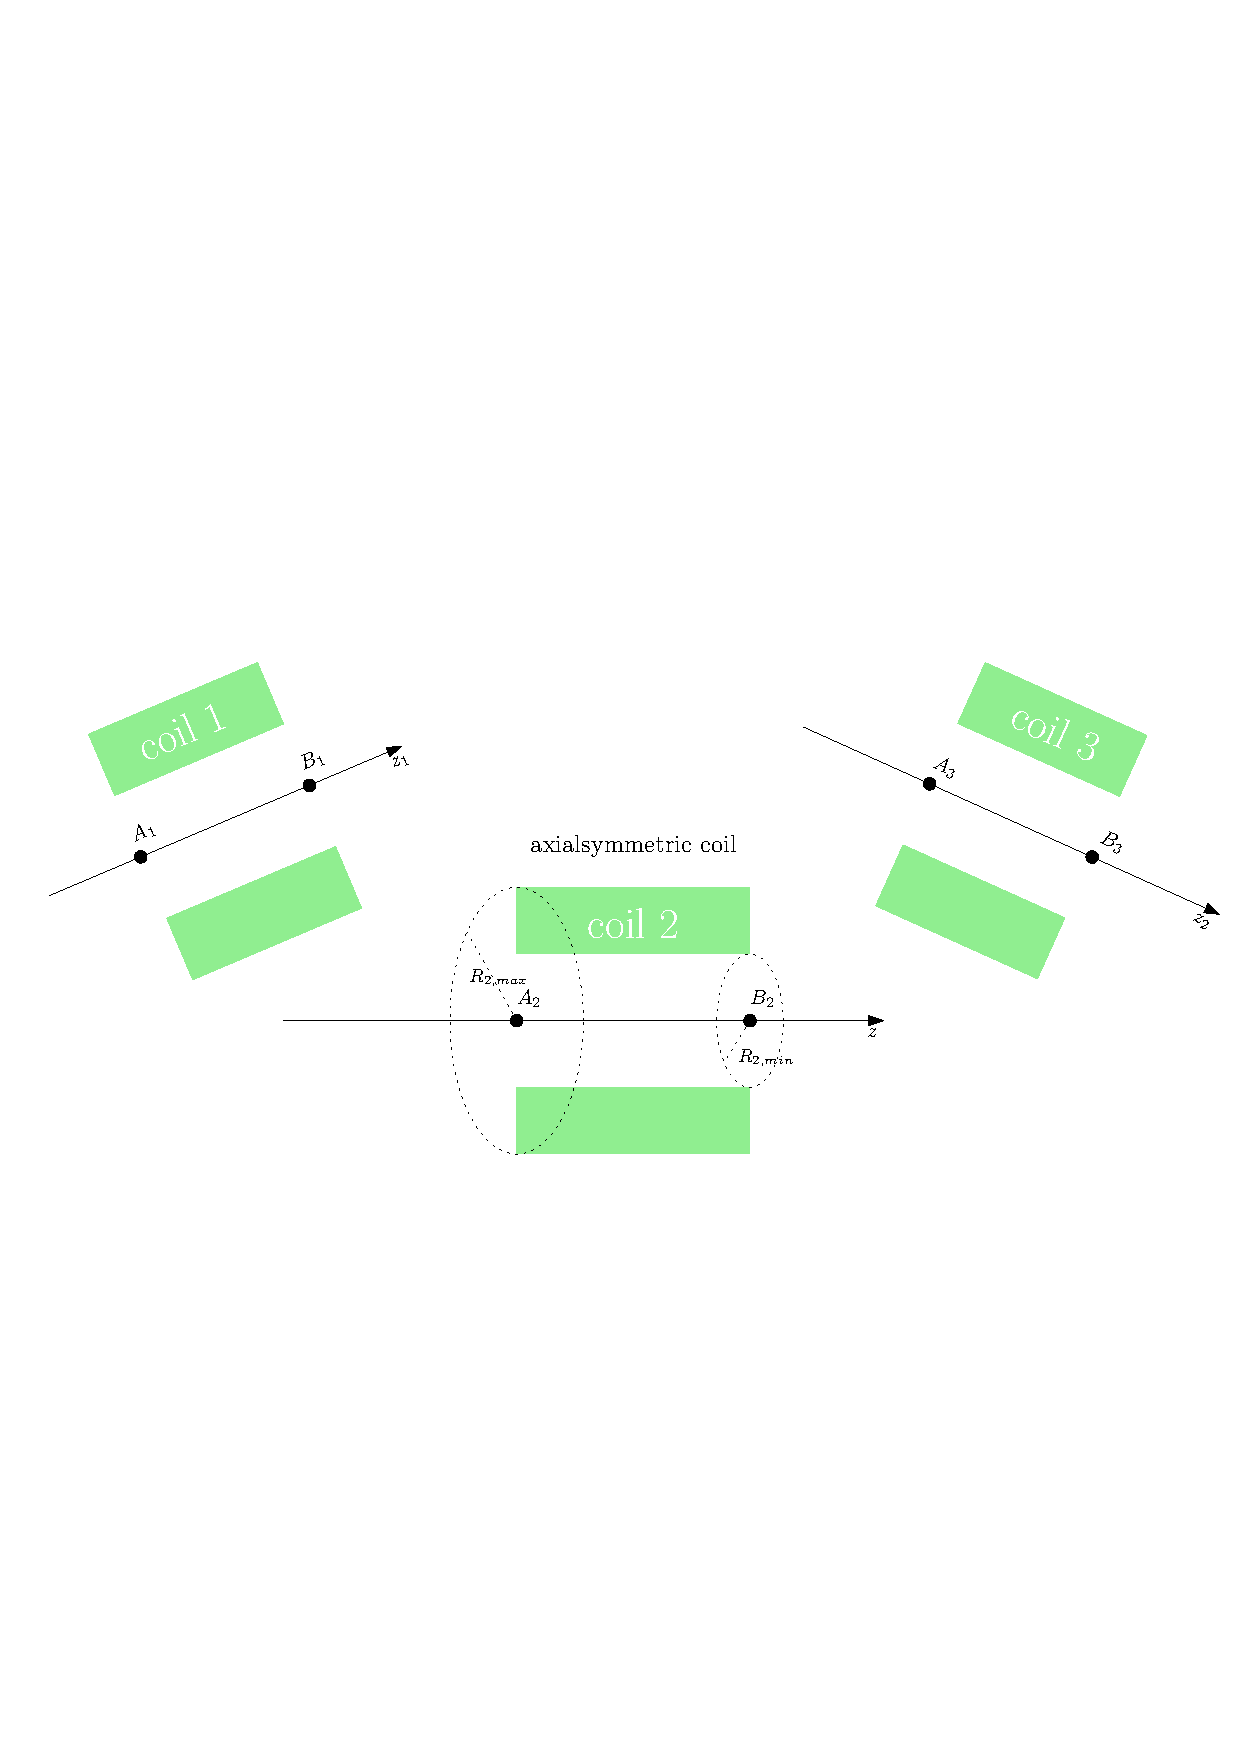
\includegraphics[width=1.0\textwidth]{images/KAFCAFigures/tilted_coils.pdf}
		\caption{Tilted coils with different symmetry axes}
	  \label{fig:tilted coils}
	\end{figure}
%% =============================
%% =============================
%% =============================
%
%
%
\subsection{Electric field calculation}
\label{ch:Methods for electric and magnetic field-calculation:sec:Electric field calculation}
  Electric field and potential calculations turn out to be more complicated than the magnetic ones. Magnetic fields are caused by electric current, a quantity which can be directly measured and set. The electric field and potential, however,  are caused by a charge distribution that is usually not known. The quantity you can set and measure on your electrodes is the voltage. The charge density on the electrodes is dependent on the voltage, but also highly dependent on the geometry of the electrode itself and on its surrounding. Another KATRIN-specific requirement is the ability to handle large volumes enclosed by electrodes. Most of the methods used to simulate electric fields, like for example the Finite Difference Method, are not applicable in such a case, as they divide the volume into a close-meshed grid, which, for extended geometries, can not be handled without serious problems regarding computer memory. \\
  Actually, a method exists that meets these requirements, the so called \textbf{B}oundary \textbf{E}lement \textbf{M}ethod.
%% =============================
	\subsection{Boundary element method}
	  Working with the boundary element method (BEM), it is assumed that on a given surface-part of the electrode the charge density is distributed homogeneously and the resulting electric field can be derived from it. Analogous to the line-segment methods discussed earlier in this chapter, the discretization into surface elements offers the ability to form any complex shape out of such elements with variable level of detail and thereby accuracy.\\
	  An electrode can be discretized into $N$ sub-elements $S_j$. The geometry $S$ can be written as a sum of these sub-elements:
	\begin{equation}
		S = \sum_{j=1}^{N} S_j
		\label{eq:sum over geometry}
	\end{equation}
	  Integrating over the charge densities $\sigma$ of all subelements, we get the potential at the position $\vec{r}$ caused by the geometry $S$ \cite{electronoptics}:
	  %potential in point r:
	  \begin{equation}
	    \Phi(\vec{r}) = \frac{1}{4\pi\varepsilon_0}\int\limits_{S}\frac{\sigma(\vec{r}_{S})}{\vert\vec{r}-\vec{r}_{S}\vert}\mathrm{d}^{2}\vec{r}_{S}
	    \label{eq:potential in point r}
	  \end{equation}
	  Although they are assumed to be constant within one subelement, the charge densities are usually not known. The quantities that are known are the voltages $U_i$, applied to the electrodes. It is possible to write down an equation system, relating the charge densities $\sigma_j$ with the voltage of the subelements $U_i$:
	  \begin{equation}
		U_{i} = \sum_{j=1}^{N} C_{ij}(\vec{r})\sigma_{j}\text{,}
		\label{eq:equation system chargedensities}
	  \end{equation}
	  with $C_{ij}=C_{j}(\vec{r}_i)$ the so called Coulomb-matrix-element. It can be seen as the electric potential at the midpoint of subelement $i$ caused by subelement $j$. It  is a geometrical factor given by:
	  \begin{equation}
		C_{j}(\vec{r}_{i}) = \frac{1}{4\pi\varepsilon_0}\int\limits_{S_j}\frac{1}{\vert\vec{r}_{i}-\vec{r}_{S}\vert}\mathrm{d}^{2}\vec{r}_{S}
		\label{eq:coulomb matrix element}
	  \end{equation}
	  The equation system \eqref{eq:equation system chargedensities} is solved using the Gauss-Jordan-algorithm, providing us with the charge densities $\sigma_j$ of the individual subelements.\\ 
	  
	  The electrodes in the KATRIN setup are in good approximation rotational symmetric. This makes it easy to describe them as cones. \\	  The electric potential of an infinitesimally thin charged ring at a field point $(z,r)$ is given by the formula:
	  \begin{equation}
	  	\Phi(z,r) = \frac{Q}{2\pi^{2}\epsilon_{0}}\frac{K(k)}{S}
	  	\label{eq:potential charged ring}
	  \end{equation}
	  where
	  \begin{equation}
	  	S = \sqrt{(R+r)^2 +(z-Z)^2}\text{,} ~~k=\frac{2\sqrt{Rr}}{S}\text{,}
	  \end{equation}
	  $Z$ is the axial coordinate of the ring, $R$ its radius, $Q$ its total charge and $K(k)$ the first complete elliptic integral (see eq. \eqref{eq:complete elliptic integrals}). \\    By numerical integration of this formula, the potential of a conical subelement with constant charge density $\sigma$ can be computed. A conical subelement, described by two points $(z_a ,r_a)$ and $(z_b,r_b)$, can be expressed as a sum of thin charged rings:
	  \begin{equation}
	  	Z= z_a +(z_b -Z_a) \cdot \frac{p}{L}\text{,} ~~R= r_a +(r_b-r_a)\cdot\frac{p}{L}\text{.}
	  \end{equation}
	  Here $p$ is the distance of the arbitrary subelement point $(Z,R)$ from the point $(z_a,r_a)$ that lies between 0 and $L$, where $L$ denotes the length of the line segment. Taking the infinitesimal charge $\mathrm{d}Q=2\pi\sigma R~\mathrm{d}p$ of the ring, the potential of the cone can finally be described:
	  \begin{equation}
	  	\Phi = \frac{\sigma}{\pi\epsilon_0}\int\limits_{0}^{L} \mathrm{d}p\frac{RK(k)}{S}
	  	\label{ep:potential conical subelement}
	  \end{equation}
	  This integral has divergences, when evaluating it close to the segment. To avoid this the integration region is divided into smaller subintervals, within which the integrand does not have any divergences.	 
	\subsection{Legendre polynomial expansion}
	  Similar to the magnetic field, the zonal harmonic expansion is applicable in case of axisymmetric electric fields. Depending on the convergence ratio, the computation by expansion is much faster than by elliptic integrals. Nevertheless, it needs the charge densities, computed by the BEM, as input parameters, in order to compute the source coefficients at the sourcepoints. \\
	  Analogous to eq. \eqref{eq:central polynomial expansion} and \eqref{eq:remote polynomial expansion} for the magnetic field, there exists a central polynomial expansion (for $\rho < \rho_{cen}$) for electric fields, given by:
	  %Legendre Polynomial central	
	  \begin{equation}
	    \begin{aligned}
		\Phi (z,r) &= \sum_{n=0}^{\infty} \phi_{n}^{cen} \left(\frac{\rho}{\rho_{cen}}\right)^{n}P_n(u) \\
		\mathcal{E}_{z}(z,r) &= -\frac{1}{\rho_{cen}} \sum_{n=0}^{\infty}(n+1) \phi_{n+1}^{cen} \left(\frac{\rho}{\rho_{cen}}\right)^{n}P_n(u) \\
		\mathcal{E}_{r}(z,r) &= \frac{s}{\rho_{cen}} \sum_{n=0}^{\infty} \phi_{n+1}^{cen} \left(\frac{\rho}{\rho_{cen}}\right)^{n}P'_n(u) \\
		&\text{with} \quad u = \cos\theta \quad \text{and} \quad s = \sin\theta
	    \end{aligned}
	    \label{eq:central polynomial expansion electric field}
	  \end{equation}
	  and a remote expansion (for $\rho > \rho_{rem}$), given by:
	  %Legendre Polynomial remote
	  \begin{equation}
	    \begin{aligned}
		\Phi (z,r)&= \sum_{n=0}^{\infty} \phi_{n}^{rem} \left(\frac{\rho_{rem}}{\rho}\right)^{n+1}P_n(u) \\
		\mathcal{E}_{z}(z,r) &= \frac{1}{\rho_{rem}} \sum_{n=1}^{\infty}n \phi_{n-1}^{rem} \left(\frac{\rho_{rem}}{\rho}\right)^{n+1}P_n(u) \\
		\mathcal{E}_{r} (z,r)&= \frac{s}{\rho_{rem}} \sum_{n=1}^{\infty} \phi_{n-1}^{rem} \left(\frac{\rho_{rem}}{\rho}\right)^{n+1}P'_n(u) %\\
		%&\text{with} \quad u = \cos\theta \quad \text{and} \quad s = \sin\theta
	    \end{aligned}
	  \label{eq:remote polynomial expansion electric field}
	  \end{equation}
	  where, again, $P_n(u)$ are the Legendre polynomials, $\phi_{n}^{rem}$ and $\phi_{n}^{cen}$ are the source coefficients at the source points and $\rho_{rem}$ and $\rho_{cen}$ are the convergence radii, given by the maximum and minimum distance from the sourcepoint to the electrode. The source coefficients $\phi_{n}^{rem}$ and $\phi_{n}^{cen}$ are determined by the surface and volume charge of the electrode \cite{Glueck2009}.
%============================
%============================
	  \subsection{Implementation}
	    \subsubsection{Magfield3}
	    \subsubsection{ELCDRing}
	    \subsubsection{ELCDCone}
	    \subsubsection{ELCDRectangle}
	    \subsubsection{ELCDWire}
